% Figure: where HOL and FOL systems pay for complexity (part 2).
% Build: pdflatex where_you_pay.tex  (run inside figures/)
\documentclass[tikz,border=6pt]{standalone}
\usetikzlibrary{positioning}
\begin{document}
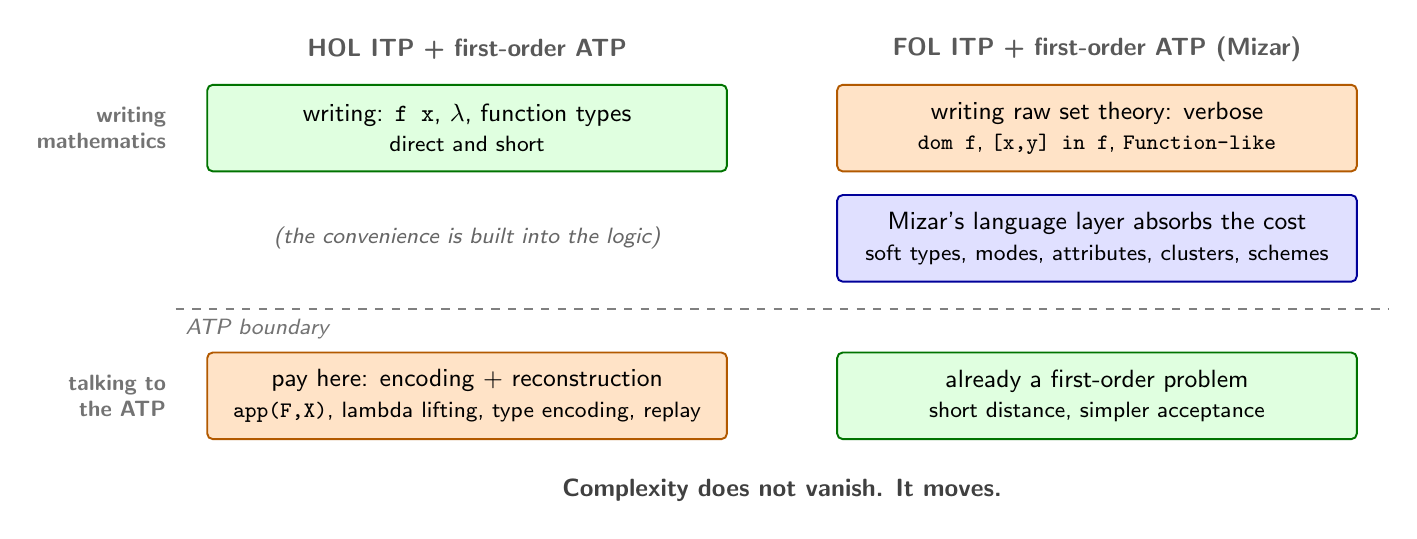
\begin{tikzpicture}[
  font=\sffamily,
  box/.style={draw, rounded corners=2pt, align=center, minimum width=66mm,
              minimum height=11mm, line width=0.7pt, font=\sffamily\small, inner sep=2mm},
  cheap/.style={box, fill=green!12, draw=green!45!black},
  pay/.style={box, fill=orange!22, draw=orange!70!black},
  lang/.style={box, fill=blue!12, draw=blue!60!black},
  head/.style={font=\sffamily\small\bfseries, text=black!65, align=center},
  side/.style={font=\sffamily\footnotesize\bfseries, text=black!55, align=right, anchor=east},
  note/.style={font=\sffamily\footnotesize\itshape, text=black!60, align=center},
]
  \node[head] at (0,0) {HOL ITP + first-order ATP};
  \node[head] at (80mm,0) {FOL ITP + first-order ATP (Mizar)};

  % writing row
  \node[cheap] (h1) at (0,-10mm)
    {writing: \texttt{f x}, $\lambda$, function types\\ \footnotesize direct and short};
  \node[pay] (f1) at (80mm,-10mm)
    {writing raw set theory: verbose\\ \footnotesize \texttt{dom f}, \texttt{[x,y] in f}, \texttt{Function-like}};

  % language layer row
  \node[note, text width=60mm] at (0,-24mm) {(the convenience is built into the logic)};
  \node[lang] (f2) at (80mm,-24mm)
    {Mizar's language layer absorbs the cost\\ \footnotesize soft types, modes, attributes, clusters, schemes};

  % ATP boundary
  \draw[dashed, black!50, line width=0.7pt] (-37mm,-33mm) -- (117mm,-33mm);
  \node[font=\sffamily\footnotesize\itshape, text=black!55, anchor=west] at (-37mm,-35.5mm) {ATP boundary};

  % ATP row
  \node[pay] (h3) at (0,-44mm)
    {pay here: encoding + reconstruction\\ \footnotesize \texttt{app(F,X)}, lambda lifting, type encoding, replay};
  \node[cheap] (f3) at (80mm,-44mm)
    {already a first-order problem\\ \footnotesize short distance, simpler acceptance};

  \node[side] at (-37mm,-10mm) {writing\\ mathematics};
  \node[side] at (-37mm,-44mm) {talking to\\ the ATP};

  \node[font=\sffamily\small\bfseries, align=center, text=black!75] at (40mm,-56mm)
    {Complexity does not vanish. It moves.};
\end{tikzpicture}
\end{document}
